\documentclass[11pt]{beamer}
\usepackage[T1]{fontenc}
\usepackage{hyperref}
\usepackage{url}
\usepackage{xcolor}
\usepackage[linesnumbered, ruled, longend]{algorithm2e}
\usepackage{colortbl}
\usepackage{subcaption}
\usepackage{amsmath,amssymb}
\usepackage{ragged2e}
\usepackage{multirow}
\usepackage{changepage}
\setbeamerfont{frametitle}{size=\large}
\usepackage{caption}
\captionsetup{labelformat=empty}
\usepackage{booktabs}
\usepackage{array}
\newcolumntype{P}{>{\centering\arraybackslash}p}
%\usepackage{enumitem}
% \usepackage[table,xcdraw]{xcolor}
% \usepackage{etoolbox}
\renewcommand{\raggedright}{\leftskip=0pt \rightskip=0pt plus 0cm}
\apptocmd{\frame}{}{\justifying}{}
\let\oldenumerate=\enumerate 
\renewenvironment{enumerate}{\oldenumerate\raggedright}{\endlist} 
\let\olditemize=\itemize
\renewenvironment{itemize}{\olditemize\raggedright}{\endlist}

\usepackage{xcolor}
\definecolor{commentgreen}{RGB}{2,112,10}
\definecolor{eminence}{RGB}{108,48,130}
\definecolor{weborange}{RGB}{255,165,0}
\definecolor{frenchplum}{RGB}{129,20,83}

\usepackage{listings}
\usepackage{textcomp}
\lstset {
	language=Java,
	frame=tb,
	tabsize=4,
	showstringspaces=false,
	numbers=left,
	upquote=true,
	commentstyle=\color{commentgreen},
	keywordstyle=\color{eminence},
	stringstyle=\color{red},
	basicstyle=\small\ttfamily, % basic font setting
	emph={int,char,double,float,unsigned,void,bool},
	emphstyle={\color{blue}},
	escapechar=\&,
	% keyword highlighting
	classoffset=1, % starting new class
	morekeywords={>,<,.,;,,,-,!,=,~},
	keywordstyle=\color{weborange},
	classoffset=0,
}

\usepackage{adjustbox}
\newcommand{\code}[1]{\texttt{#1}}

\usetheme{Warsaw}
%\useoutertheme{smoothtree}
\usepackage[utf8]{vietnam}
%%%%%%%%%%%%%%%%%%%%%%%%%%%%%%%%%%%%
\def\mydate{\leavevmode\hbox{\bfseries\the\day/\twodigits\month/\twodigits\year}}
\def\twodigits#1{\ifnum#1<10 0\fi\the#1}
%%%%%%%%%%%%%%%%%%%%%%%%%%%%%%%%%%%%
\definecolor{sectioncolor}{RGB}{39,0,118}
\definecolor{framecolor}{RGB}{37,109,255}

\setbeamercolor{frametitle}{fg=white, bg=blue}
\definecolor{light-gray}{gray}{0.95}
%%%%%%%%%%%%%%%%%%%%%%%%%%%%%%%%%%%
\setbeamertemplate{footline}
{%
	\leavevmode%
	\begin{beamercolorbox}[wd=.5\paperwidth,ht=2.75ex,dp=1.5ex]{author in head/foot}%
		\hbox to .5\paperwidth{\hfil\insertshortauthor\hfil}
	\end{beamercolorbox}%
	\begin{beamercolorbox}[wd=.5\paperwidth,ht=2.75ex,dp=1.5ex]{date in head/foot}%
		\raggedleft
		\usebeamerfont{date in head/foot}
		\insertframenumber{} / \inserttotalframenumber\hspace*{15pt}
	\end{beamercolorbox}%
}
%==============================================
\makeatletter
\patchcmd{\beamer@sectionintoc}
{\vfill}
{\vskip\itemsep}
{}
{}
\makeatother  
\begin{document}
\captionsenglish
\dateUSenglish
\author[Le Vu Loi]{
	\begin{center}
		{\bfseries\fontsize{16pt}{\baselineskip}\selectfont DISTRIBUTED TRAINING} \\[10pt]
		{Author. Le Vu Loi}
	\end{center}
}
	\title[]{\bfseries\fontsize{14}{\baselineskip}\selectfont Seminar Lab AI\vspace{5pt}}
%	\subtitle{\fontsize{16}{\baselineskip}\selectfont DISTRIBUTED TRAINING}
%	\logo{\includegraphics[scale=.1]{images/SoICTlogo.jpg}}
	\institute[\bfseries CMC ATI]{}
	\date[\mydate]{\today}
	%\subject{Yo!}
	
\begin{frame}[plain]
	\maketitle
\end{frame}
\begin{frame}[plain]
	\frametitle{Outline}
	\tableofcontents
\end{frame}
% ======
\section{Categorization of distributed training}
\frame{\tableofcontents[currentsection]}
\begin{frame}
\frametitle{Categorization of distributed training}
\begin{itemize}
	\item Data parallelism
	\begin{itemize}
	\item \textit{Synchronous:} In sync training, all workers train over different slices of input data in sync, and aggregating gradients at each step.
	\item \textit{Asynchronous:} In async training, all workers are independently training over the input data and updating variables asynchronously.
	\item Typically sync training is supported via all-reduce and async through parameter server architecture.
	\end{itemize}
	\item Model parallelism
	\item Pipeline parallelism: combine data and model parallelism.
\end{itemize}
\end{frame}
% ======
\begin{frame}
\frametitle{Data parallelism}
\begin{columns}[c]
\begin{column}{.6\textwidth}
\begin{itemize}
	\item A batch of data is sharded into multiple shards.
	\item Each shard of a batch is run on a training device. (TPU/GPU).
\end{itemize}
\end{column}
\begin{column}{.4\textwidth}
\begin{center}
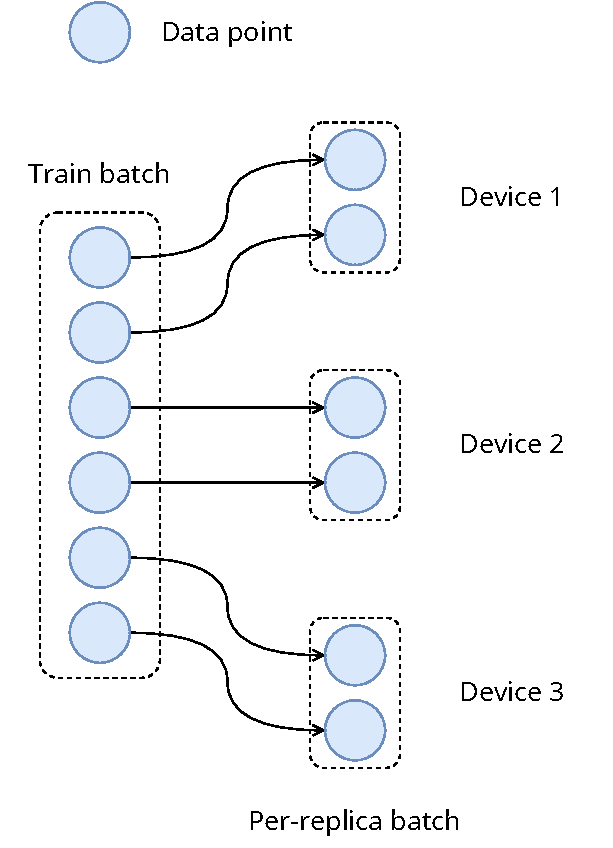
\includegraphics[scale=.4]{images/model/data-parallel-Page-1.drawio.pdf}
\end{center}
\end{column}
\end{columns}
\end{frame}
% ======
\begin{frame}
\frametitle{Synchronous data parallelism}
\begin{itemize}
\item Each training device holds a copy of model parameters. All model replicas are kept in sync.
\item Each training device runs with a shard of input data. The computed gradients on each device are then aggregated before performing an update.
\end{itemize}
\end{frame}
% ======
\begin{frame}
\frametitle{Asynchronous data parallelism: Parameter server architecture}
\begin{figure}
	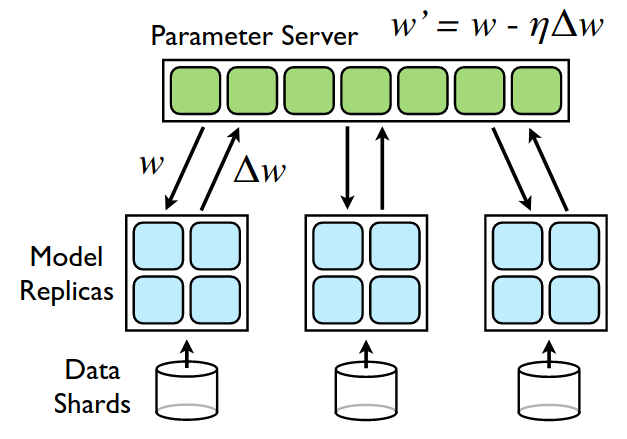
\includegraphics[scale=.3]{images/model/arch-param-server.png}
\end{figure}
\end{frame}
% ======
\begin{frame}
	\frametitle{Asynchronous data parallelism: Parameter server architecture}
	\begin{itemize}
		\item The most up-to-date gold-standard parameters are the ones stored in memory on the \textbf{parameter server}.
		\item The parameter server updates its parameters by using gradients that are computed by the other machines, known as \textbf{workers}.
		\item Workers pull parameters from parameter server before a forward, and push gradients to parameter server after a backward.
	\end{itemize}
\end{frame}
% ======
\begin{frame}
\frametitle{Asynchronous data parallelism: Parameter server architecture}
\framesubtitle{Worker pseudocode}
\begin{figure}
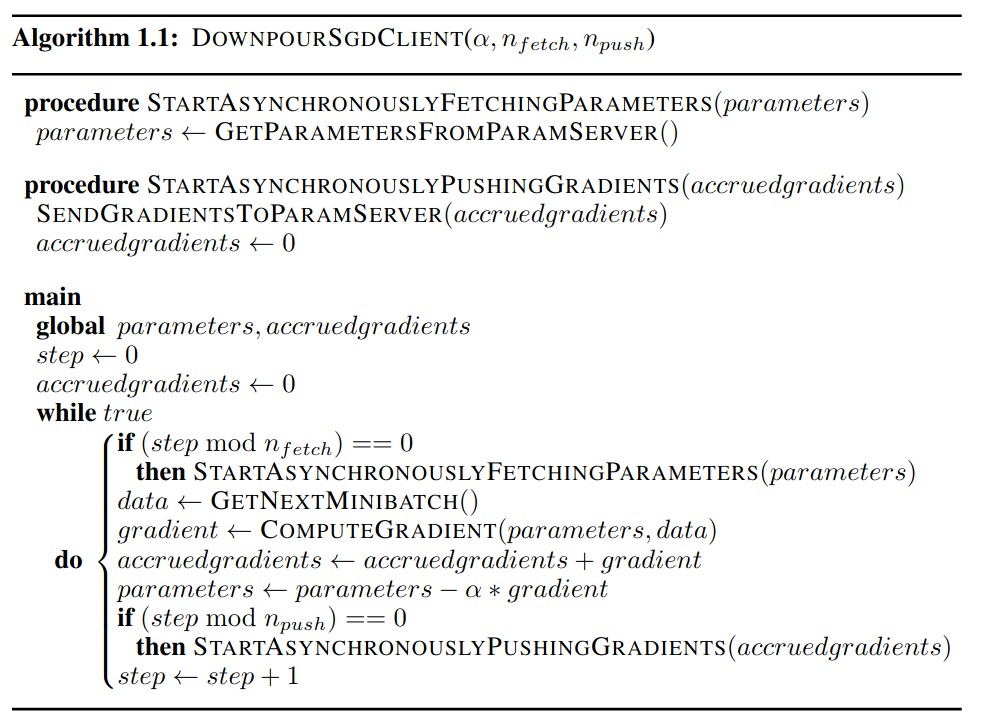
\includegraphics[scale=.25]{images/model/client-code-param-server.png}
\end{figure}
\end{frame}
% ======
\begin{frame}
\frametitle{Model parallelism in PyTorch}
\begin{center}
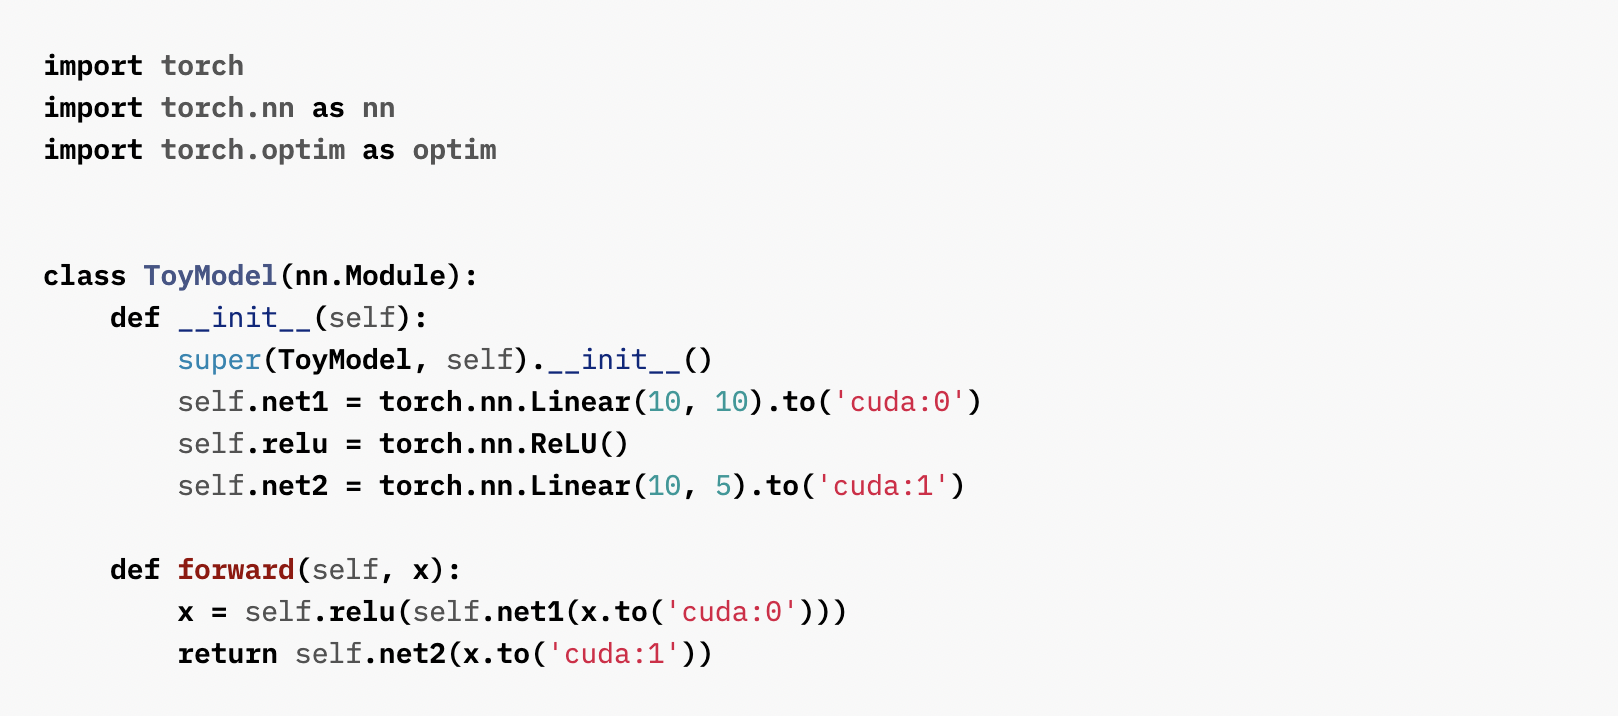
\includegraphics[scale=.3]{images/code/parallelize-model.png}
\end{center}
\begin{itemize}
	\item Labels need to be on the same device as the outputs when calling loss function.
	\item \texttt{backward()} and \texttt{torch.optim} automatically take care of gradients as if the model is on one GPU.
\end{itemize}
\end{frame}
% ======
\begin{frame}
\frametitle{Parallelize model in PyTorch}
\framesubtitle{Speed up by pipelining inputs}
\begin{itemize}
	\item Given 4 GPUs, a model $M$ which spans these 4 GPUs and contains 4 modules: $M_0$, $M_1$, $M_2$, $M3$, where $M_i$ resides on the $i$-th GPU.
	\item A batch of samples $A$, which is splitted into 4 chunks: $A_0$, $A_1$, $A_2$, $A_3$.\\[10pt]
	\item Let $r^{(i)}_j = M_j(A_i)$
\end{itemize}
\end{frame}
% ======
\begin{frame}
	\frametitle{Parallelize model in PyTorch}
	\framesubtitle{Speed up by pipelining inputs: Demonstration}
	\only<1>{
		\begin{figure}[h]
			\centering
			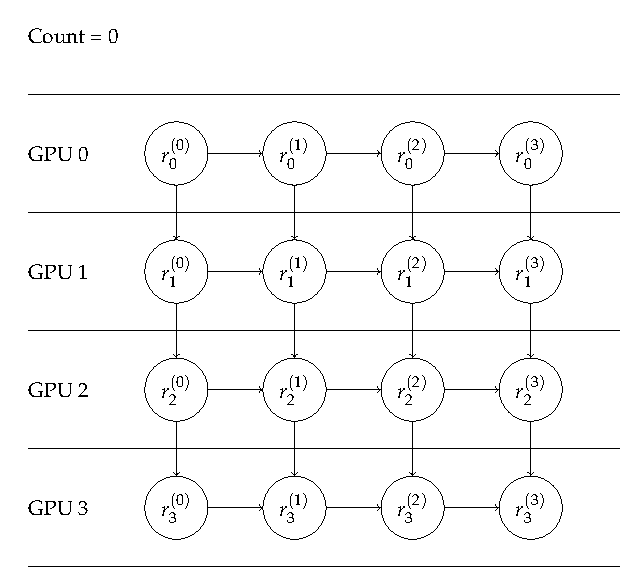
\includegraphics[scale=0.7]{images/orders/count/count0.pdf}
			\label{fig:00}
		\end{figure}
	}
	\only<2>{
		\begin{figure}[h]
			\centering
			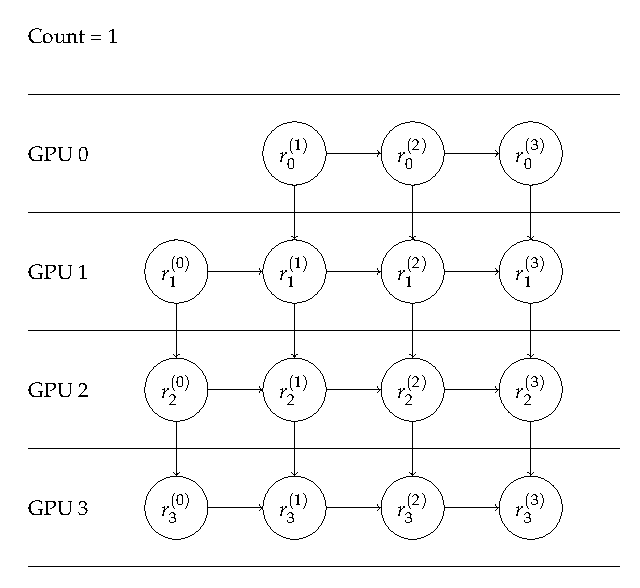
\includegraphics[scale=0.7]{images/orders/count/count1.pdf}
			\label{fig:01}
		\end{figure}
	}
	\only<3>{
		\begin{figure}[h]
			\centering
			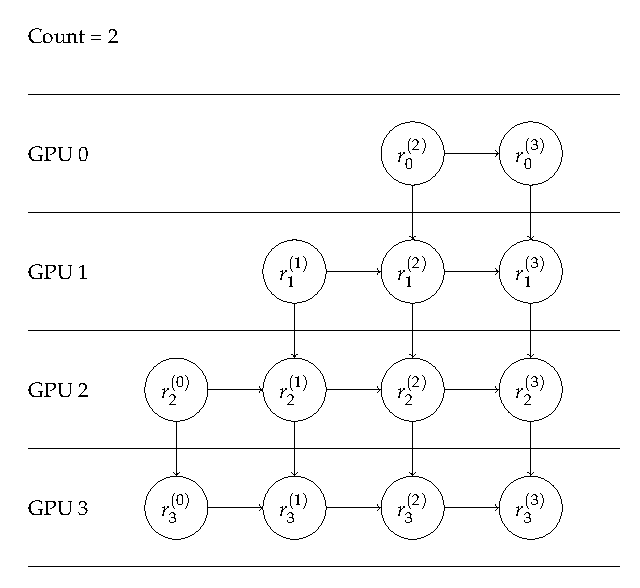
\includegraphics[scale=0.7]{images/orders/count/count2.pdf}
			\label{fig:02}
		\end{figure}
	}
	\only<4>{
	\begin{figure}[h]
		\centering
		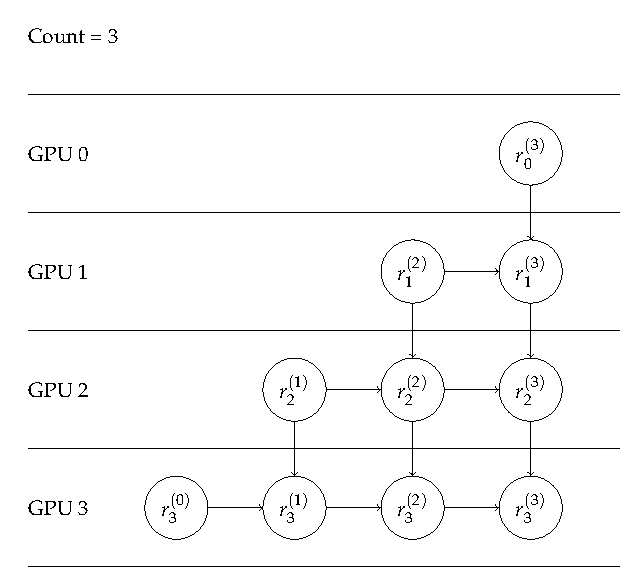
\includegraphics[scale=0.7]{images/orders/count/count3.pdf}
		\label{fig:03}
	\end{figure}
}
	\only<5>{
	\begin{figure}[h]
		\centering
		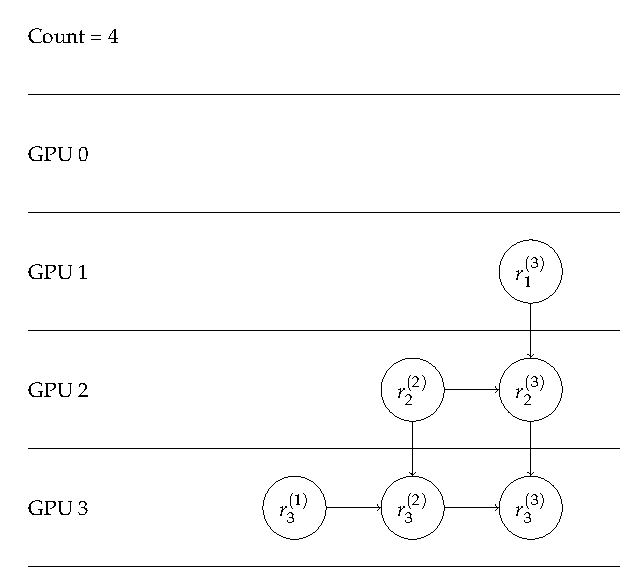
\includegraphics[scale=0.7]{images/orders/count/count4.pdf}
		\label{fig:04}
	\end{figure}
}
	\only<6>{
	\begin{figure}[h]
		\centering
		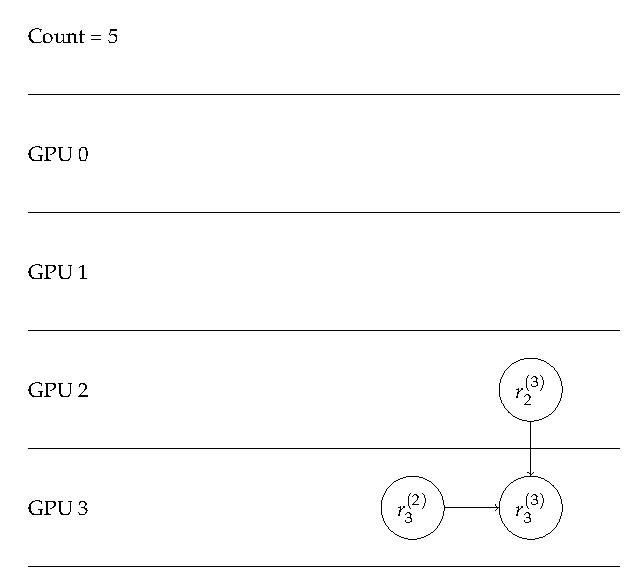
\includegraphics[scale=0.7]{images/orders/count/count5.pdf}
		\label{fig:05}
	\end{figure}
}
	\only<7>{
	\begin{figure}[h]
		\centering
		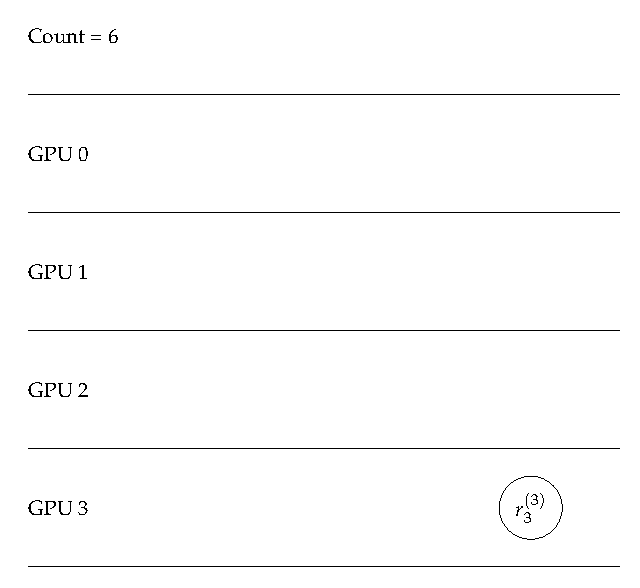
\includegraphics[scale=0.7]{images/orders/count/count6.pdf}
		\label{fig:06}
	\end{figure}
}
	\only<8>{
	\begin{figure}[h]
		\centering
		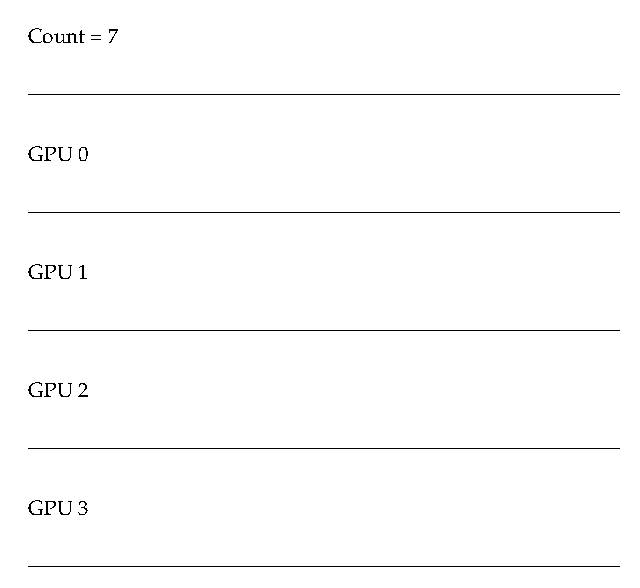
\includegraphics[scale=0.7]{images/orders/count/count7.pdf}
		\label{fig:07}
	\end{figure}
}
\end{frame}
% ======
\begin{frame}
	\frametitle{Comparisons of different distributed training strategy}
	\begin{itemize}
		\item Data parallelism is more commonly used than model parallelism, it is quite straightforward to set up
		\item Model parallelism usually requires delicate design of device connection and model partition.
		\item Asynchronous execution has been largely replaced by synchronous execution. This is mostly due to concerns about model stability and convergence.
	\end{itemize}
\end{frame}
% ======
\section{Distributed training in Tensorflow}
\frame{\tableofcontents[currentsection]}
% ======
\begin{frame}
\frametitle{Distributed training in Tensorflow}
\begin{itemize}
	\item Common distributed strategies in Tensorflow includes:
	\begin{itemize}
		\item \texttt{MirroredStrategy}: one node, multiple GPUs per node.
		\item \texttt{MultiWorkerMirroredStrategy}: multiple nodes, multiple GPUs per node.
		\item \texttt{TPUStrategy}: the same as the 2 above strategies but for TPUs.
	\end{itemize}
\end{itemize}
\end{frame}
% ======
\begin{frame}
\frametitle{Distributed training in Tensorflow}
\framesubtitle{Data Loader}
\begin{itemize}
\item The \texttt{tf.data.Dataset} class supports efficient input data pipeline. It can also be used in distributed training to distribute data to multiple training devices.
\item To use \texttt{tf.data.Dataset} in distributed training, it is as simple as adding just one line of code.
\item Data is produced on CPU and is consumed by GPUs, i.e. one producer, multiple consumers.
\end{itemize}
\end{frame}
% ======
\begin{frame}
\frametitle{Distributed training in Tensorflow}
\framesubtitle{Code pattern}
\begin{columns}[c]
\begin{column}{.5\textwidth}
\begin{figure}[!h]
\centering
\caption{Initialize a distributed strategy}
\vspace*{-15pt}
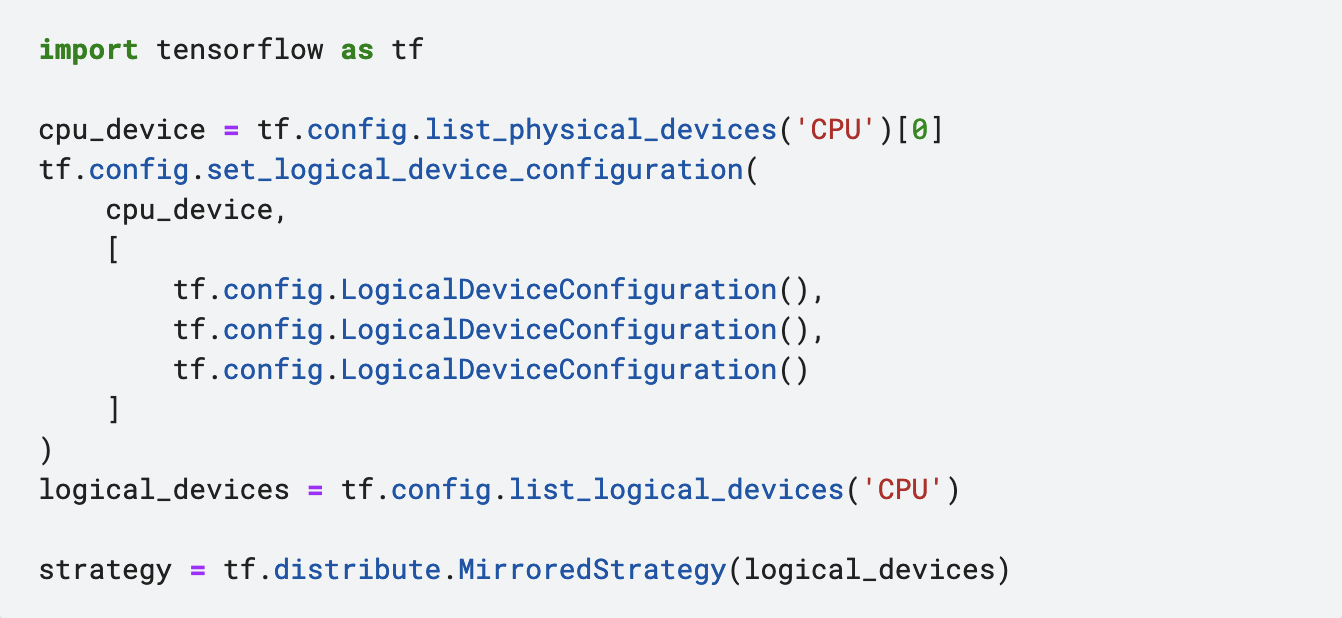
\includegraphics[scale=0.23]{images/code/tf-strategy.png}
\end{figure}
\vspace*{-15pt}
\begin{figure}[!h]
\centering
\caption{Training loop}
\vspace*{-15pt}
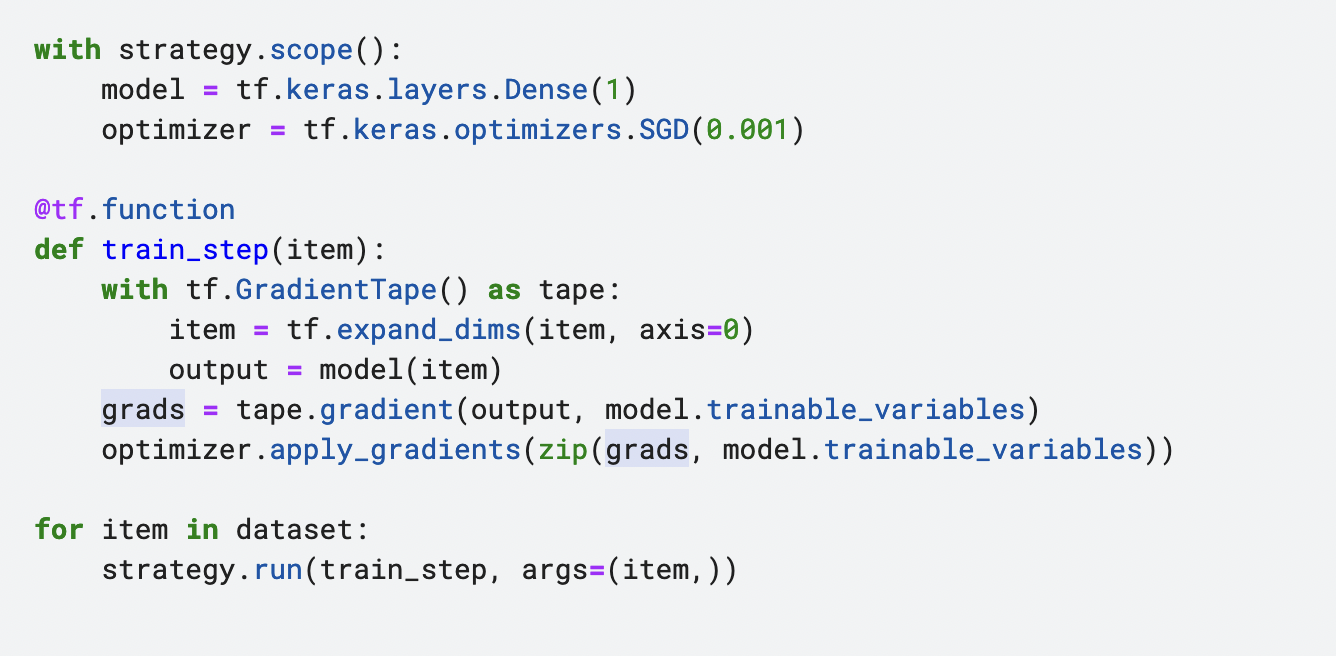
\includegraphics[scale=.23]{images/code/train-loop-tf.png}
\end{figure}
\end{column}
\begin{column}{.5\textwidth}
\begin{figure}[!h]
	\centering
	\caption{Distribute a dataset}
	\vspace*{-15pt}
	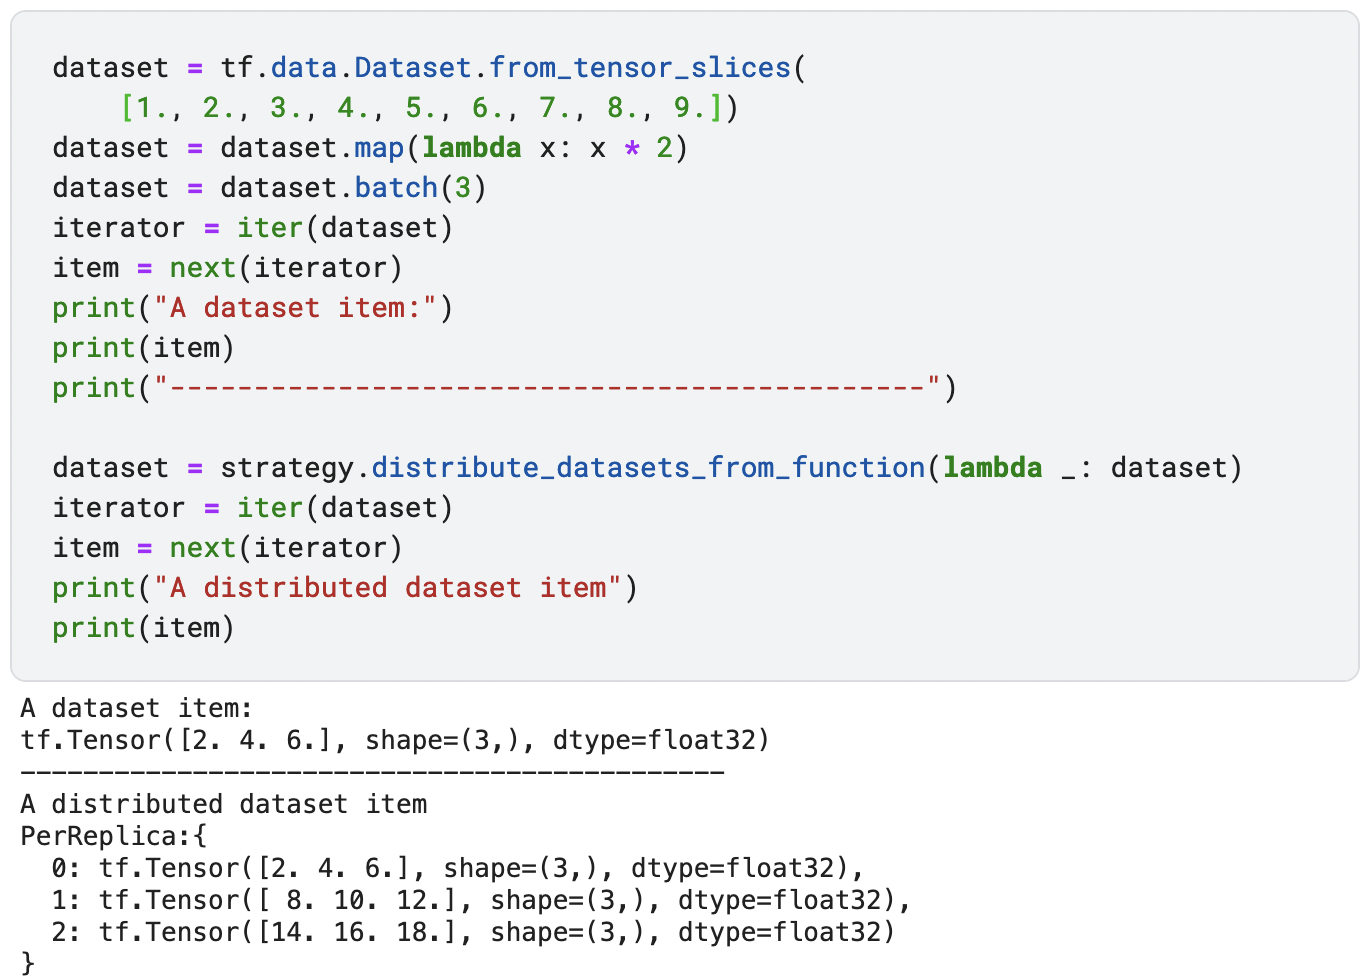
\includegraphics[scale=0.23]{images/code/dist-dataset.png}
\end{figure}
\end{column}
\end{columns}
\end{frame}
% ======
\section{Distributed training in PyTorch}
\frame{\tableofcontents[currentsection]}
\begin{frame}
\frametitle{Types of distributed training in PyTorch}
\begin{itemize}
	\item Data parallel training
	\item Distributed data parallel training
	\item RPC-based distributed training
\end{itemize}
\end{frame}
% ======
\begin{frame}
\frametitle{Data parallel}
\begin{itemize}
	\item \texttt{torch.nn.DataParallel} offers minimal code changes to switch to distributed training.
	\item To use \texttt{torch.nn.DataParallel}, simply wrap a model in it.
	\item \texttt{torch.nn.DataParallel} uses multi thread for distributed training.
\end{itemize}
\end{frame}
% ======
\begin{frame}
\frametitle{Data parallel}
\framesubtitle{Code pattern}
\begin{figure}[!h]
\centering
\caption{Distributed training with DataParallel}
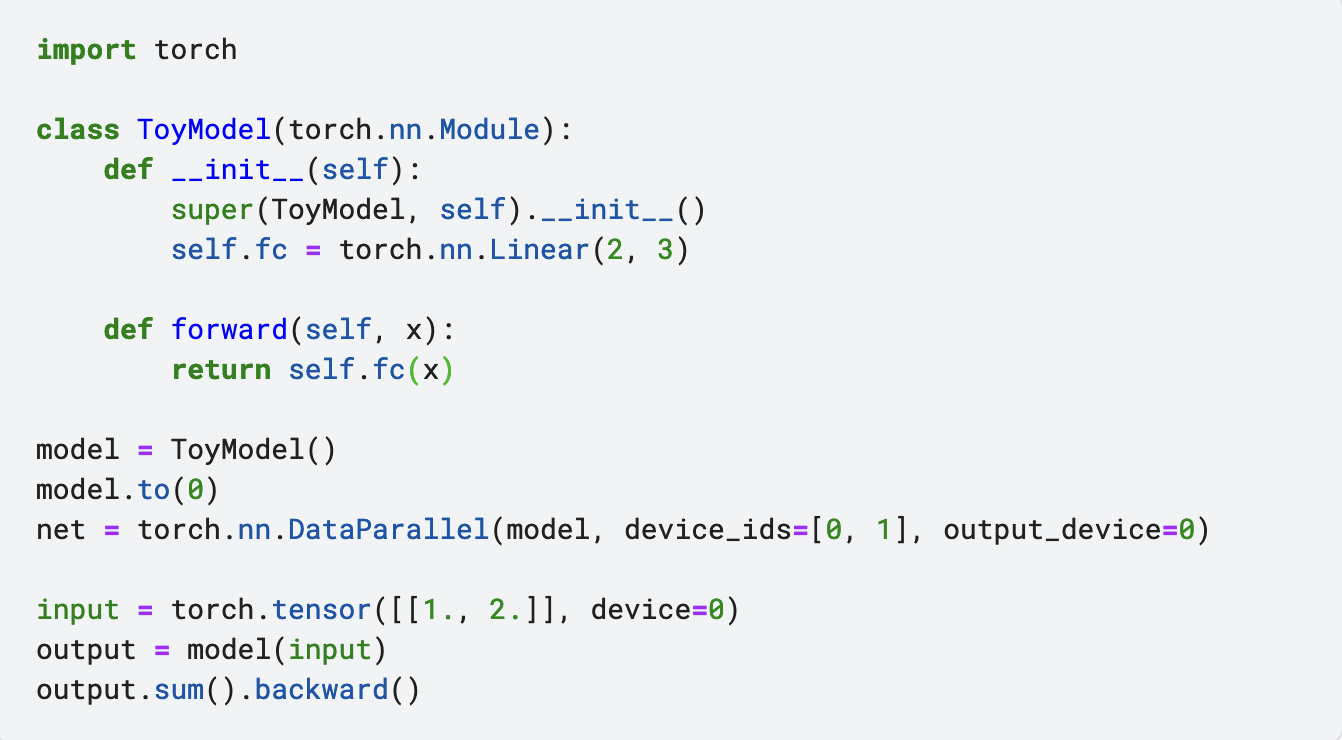
\includegraphics[scale=0.3]{images/code/torch-data-par.png}
\end{figure}
\end{frame}
% ======
\begin{frame}
\frametitle{Distributed data parallel}
\begin{itemize}
	\item Distribute training using multiprocessing.
	\item Lauch one process per GPU, each process has a rank.
	\item Data loader runs separately on each process. Thus, each process needs to get its data shard based on its rank.
\end{itemize}
\end{frame}
% ======
\begin{frame}
\frametitle{Distributed data parallel}
\framesubtitle{Code pattern}
\begin{figure}[!h]
\centering
\caption{Distributed training using DistributedDataParallel}
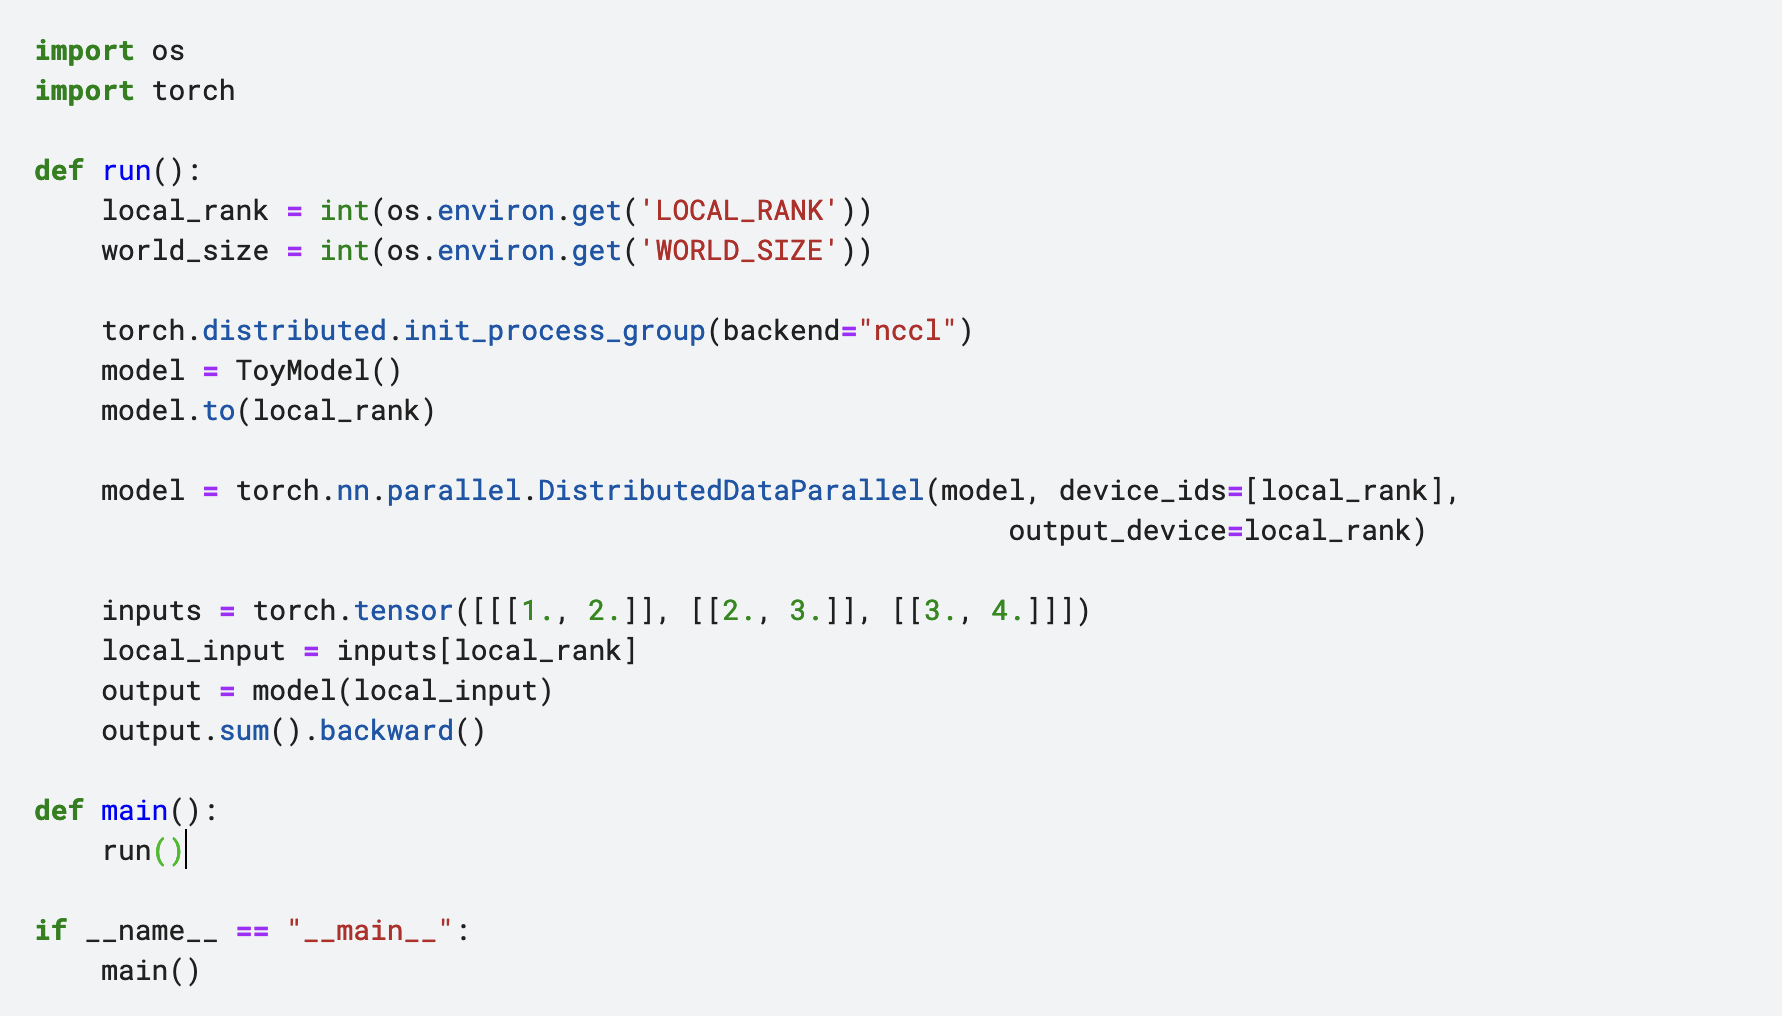
\includegraphics[scale=.3]{images/code/torch-ddp.png}
\end{figure}
\end{frame}
% ======
\section{Reproduction in distributed training}
\frame{\tableofcontents[currentsection]}
\begin{frame}
\frametitle{Reproduction in distributed training in PyTorch}
\begin{itemize}
	\item PyTorch allows to save and restore random number generation state (RNG state). Thus, the training process can be perfectly reproduced given the following information:
	\begin{itemize}
		\item Model weights
		\item Optimizer and scheduler state
		\item Data loader state
		\item Random number generator state
		\item Hardwares
	\end{itemize}
	\item Tensorflow does not allow to get the RNG state, thus it is difficult to produce perfectly reproducible results.
	\item To allow reproducible results for distributed training in PyTorch, we only need to save RNG states of all GPUs.
\end{itemize}
\end{frame}
\end{document}